\documentclass[12pt, a4paper]{article}

\title{Cutoff Finder user manual}

\author{
  Budczies, Jan
  \and
  Oliveira, Cristiano
}

\usepackage{Sweave}
\usepackage[bf]{caption}
\usepackage[utf8]{inputenc}
\usepackage{listings} % To include R code
\usepackage{graphicx} % To import png
\graphicspath{ {./} }

\begin{document}

\maketitle

\vspace{0.5cm}

\tableofcontents


\newpage

\begin{figure}[t]
\centering
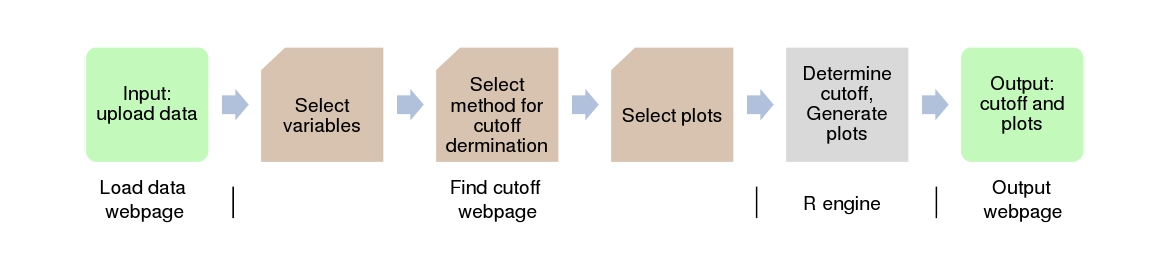
\includegraphics[width=0.9\textwidth]{fig1_workflow}
\caption{\textbf{Workflow of Cutoff Finder.} The track below the icons refers to the places where the steps of data processing are done.}
\label{fig:workflow}
\end{figure}

% ADDED by CRISTIANO
\begin{figure}[t]
\centering
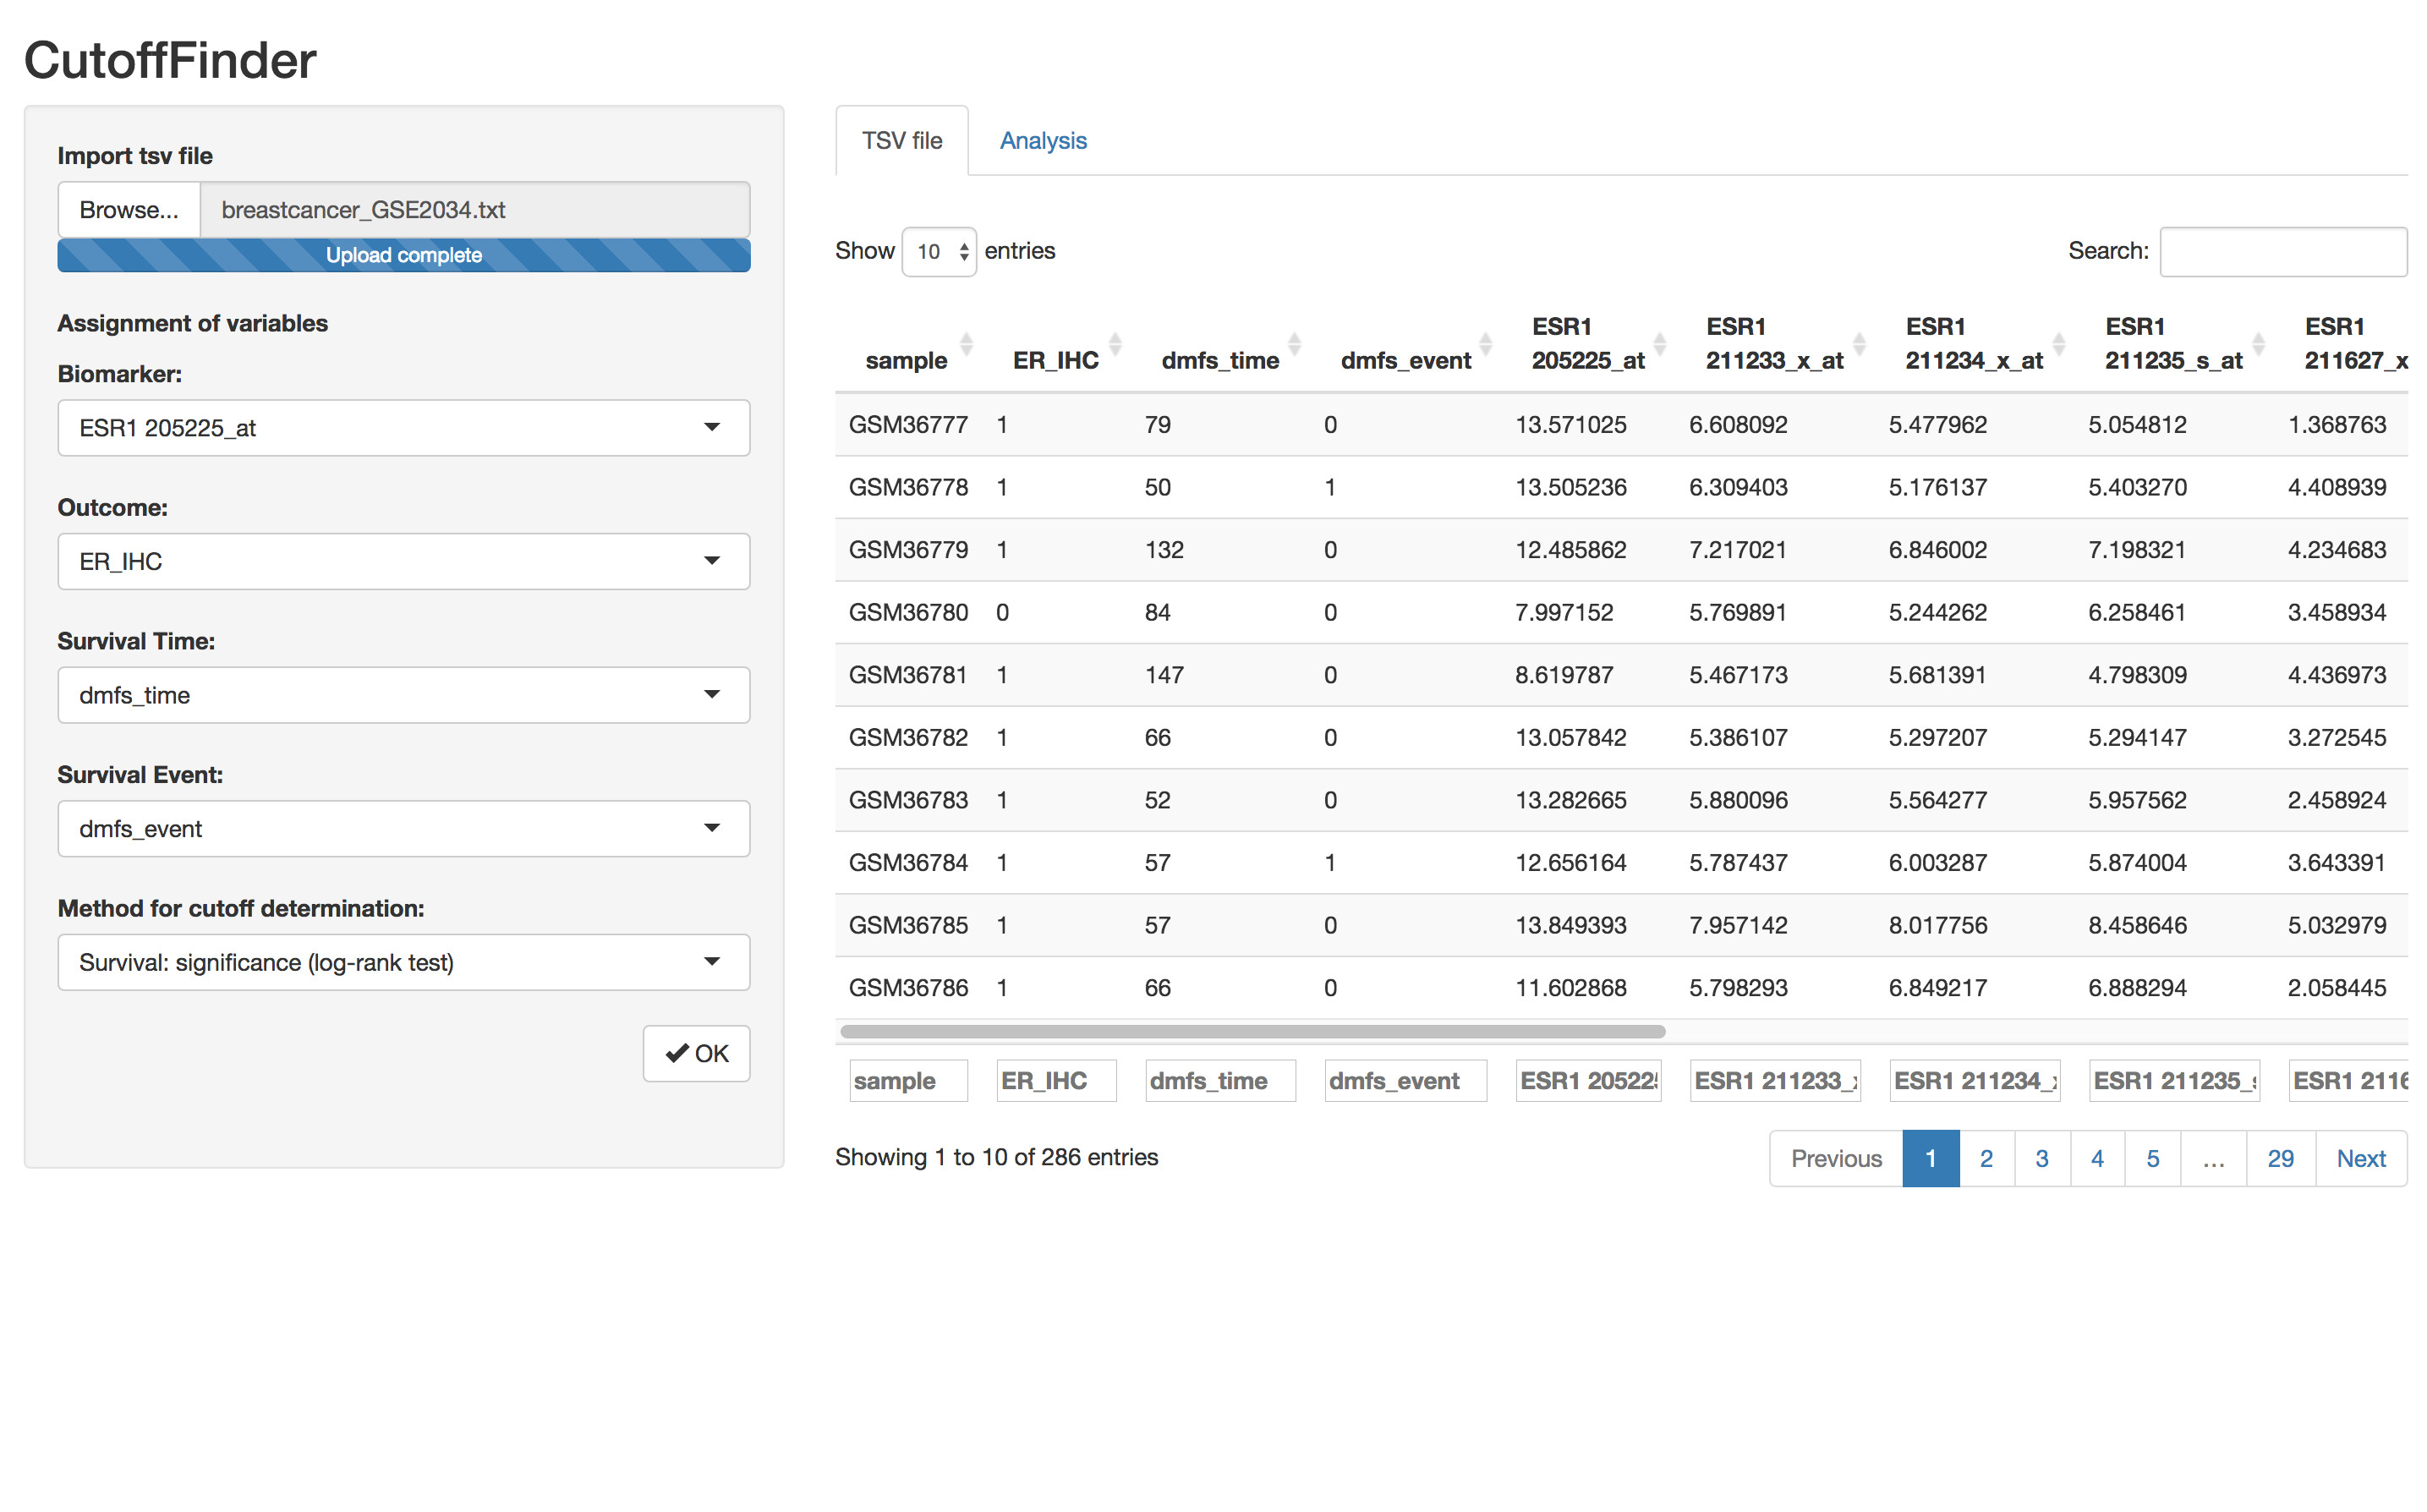
\includegraphics[width=0.9\textwidth]{cutoffFinderInput}
\caption{\textbf{cutoffFinder Input} The view with the input parameters.}
\label{fig:cutoffFinderInput}
\end{figure}

\begin{figure}[t]
\centering
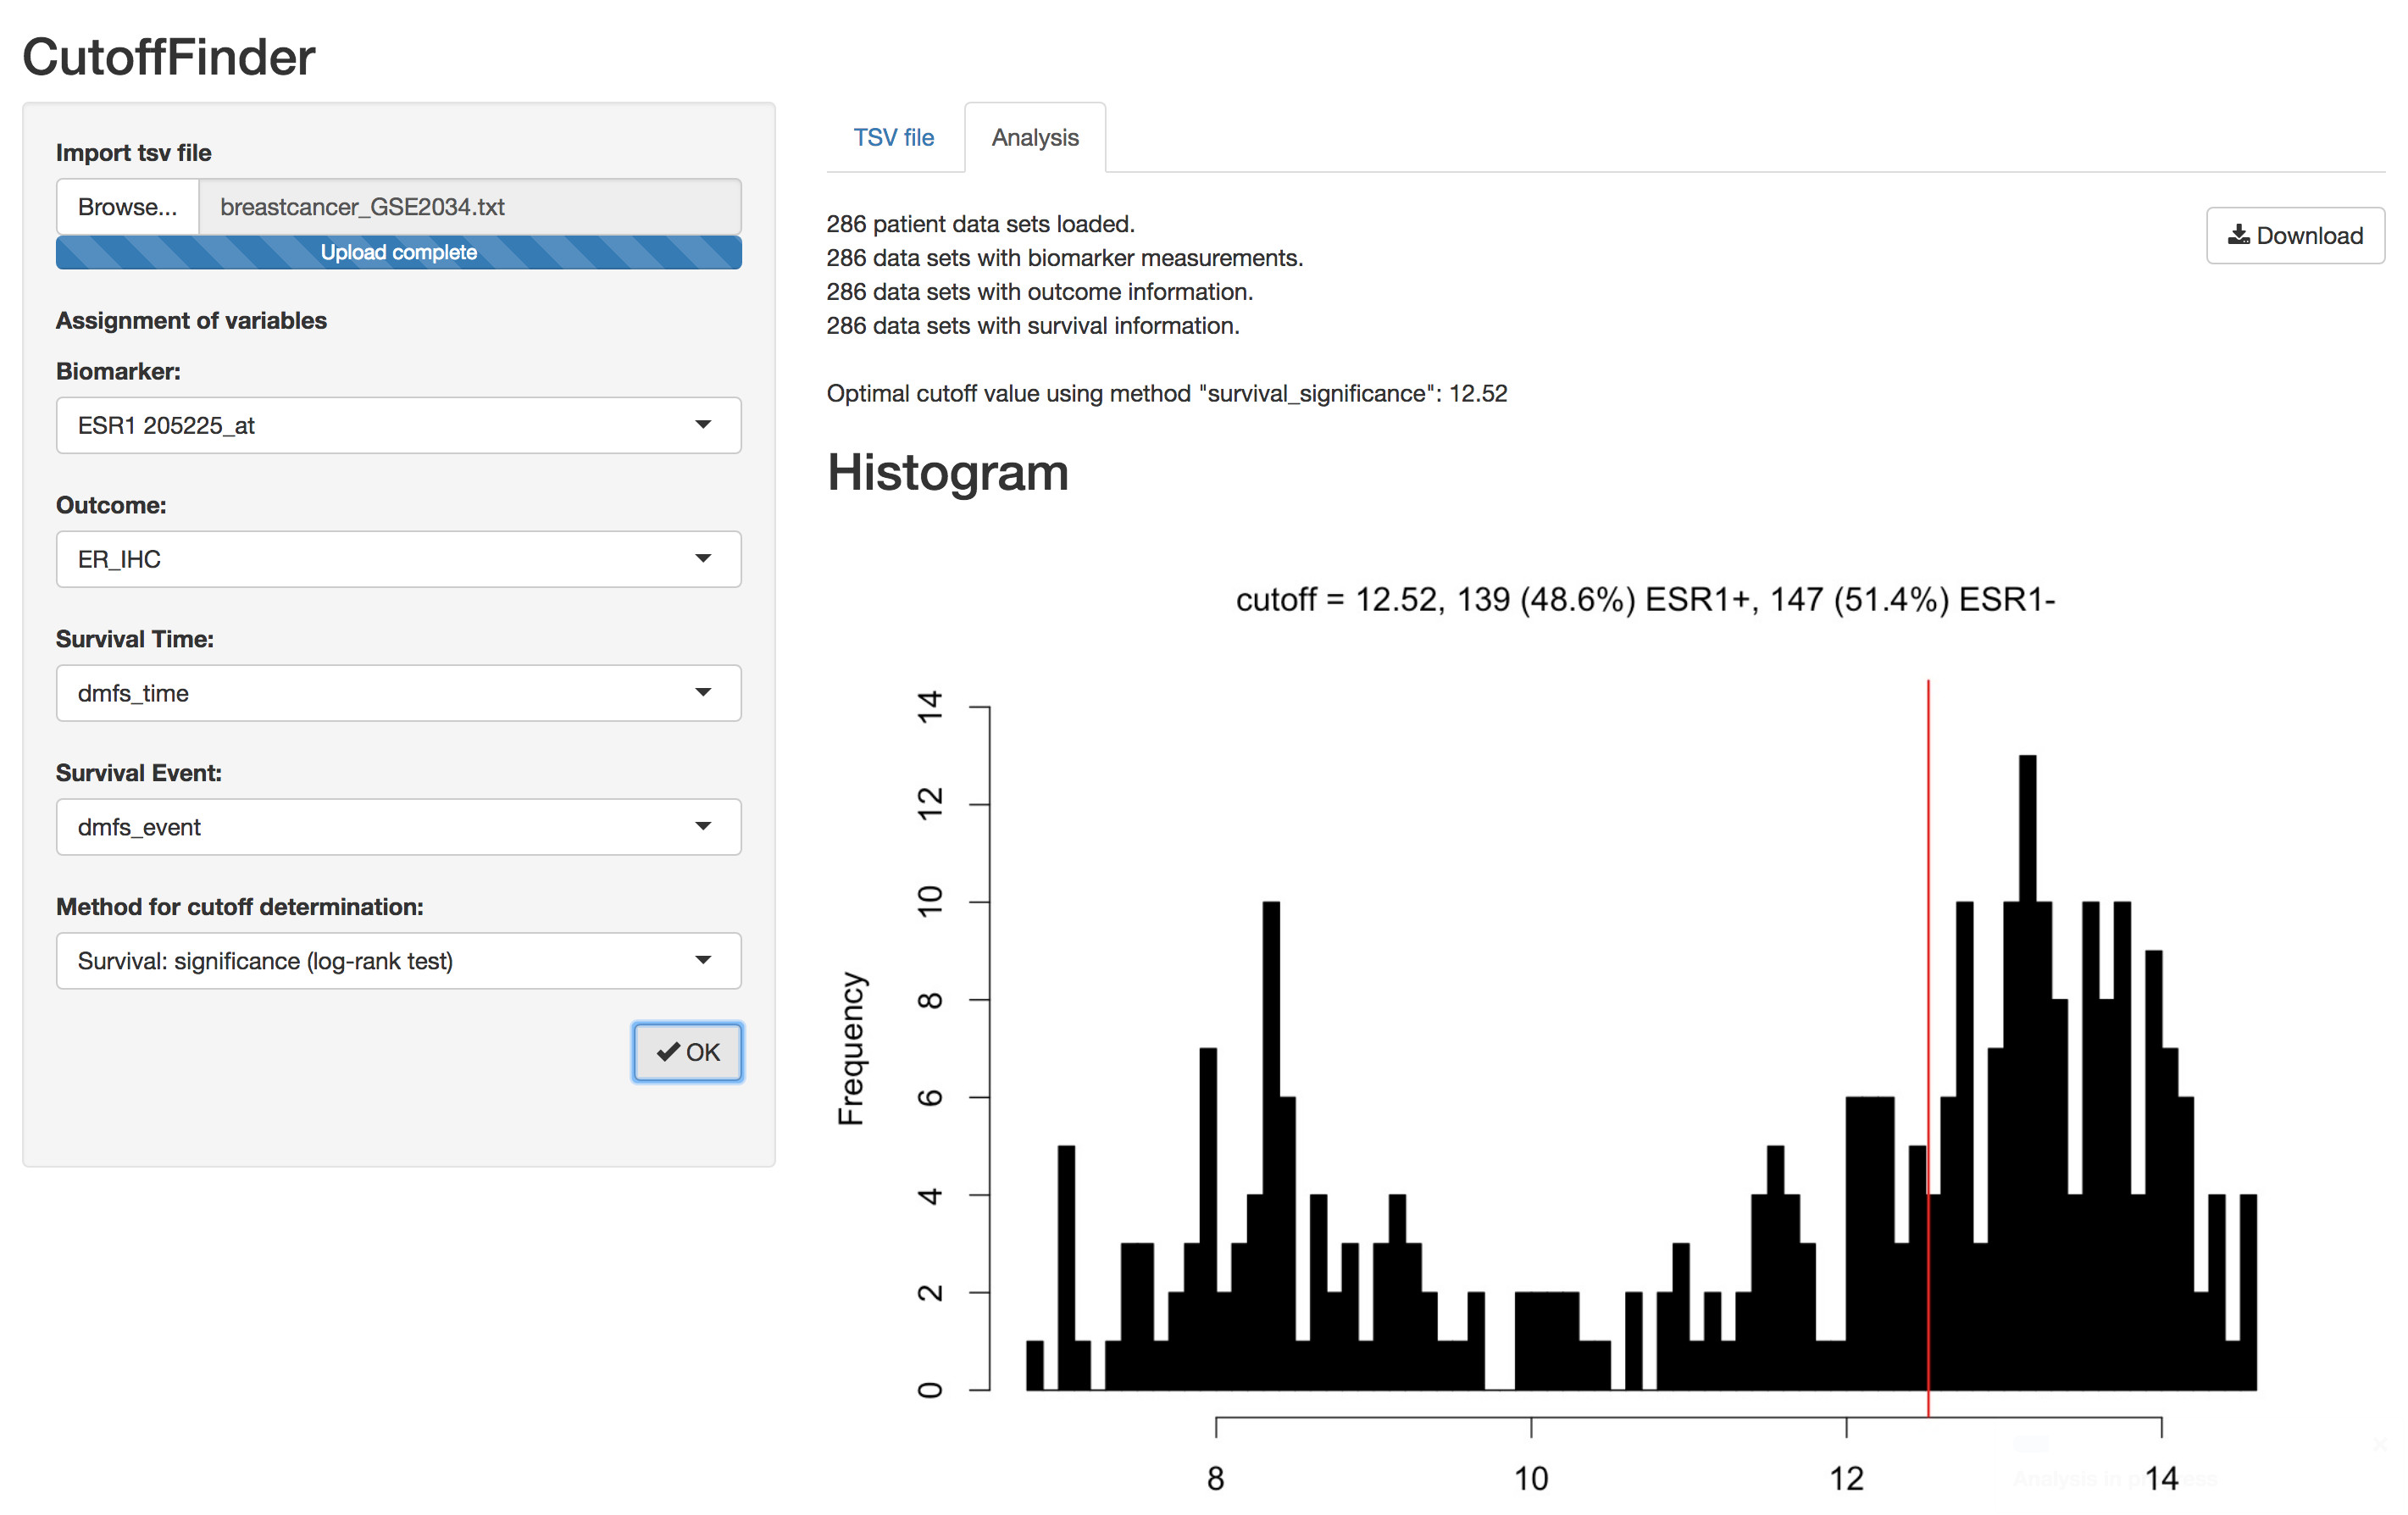
\includegraphics[width=0.9\textwidth]{cutoffFinderOutput}
\caption{\textbf{cutoffFinder Output} The view with the output parameters.}
\label{fig:cutoffFinderOutput}
\end{figure}


\section{Introduction}
Cutoff Finder is a comprehensive and easy-to-use web application for the optimization of cutoff points in molecular data.
The web application is freely available at \textbf{http://molpath.charite.de/cutoff}.
Plots generated by Cutoff Finder can be used in scientific publications, but you are kindly asked to cite \cite{Budczies2012}.

Often, molecular data such as gene expression or protein expression data are represented by continuous or at least ordinal variables.
In order to translate these variables into a clinical decision, it is necessary to determine a cutoff point and to stratify patients into two groups, each of which requiring a different kind of treatment.
Cutoff Finder offers a multitude of methods for cutoff determination and plots.
The steps of data procession are shown in Figure~\ref{fig:workflow}:

\begin{enumerate}
\item The data are uploaded from a tab-separated file, rows representing patients and columns representing variables.
Alternatively, one of three example data sets can be imported.
\item The user selects the biomarker and optionally outcome and survival variables from the table columns.
\item The user selects the method for cutoff determination.
\item The user chooses the set of plots to be generated.
\item The inquiry is send to the statistical engine R.
The optimal cutoff point is determined and analysis plots are generated.
\item The user is directed to the results webpage, where cutoff point and plots are shown.
\end{enumerate}
Each of the step is discussed in detail in the next sections.

The left part of Figure~\ref{fig:screenshot} shows the menu structure of Cutoff Finder.
\emph{Documentation} is a link to this manual.
\emph{Example data} links to three breast cancer example data sets that can be imported.
\emph{Load data} is the entry point for upload of own data.
\emph{Find cutoff} is the central webpage of the application where the user selects the variables for analysis, the method for cutoff optimization and the set of plots to be generated.
The content of the \emph{Find cutoff} webpage is shown at the right part of Figure~\ref{fig:screenshot}.
\emph{Contact} links to the authors of the webpage and the funding sources.

\begin{figure}[t]
\centering
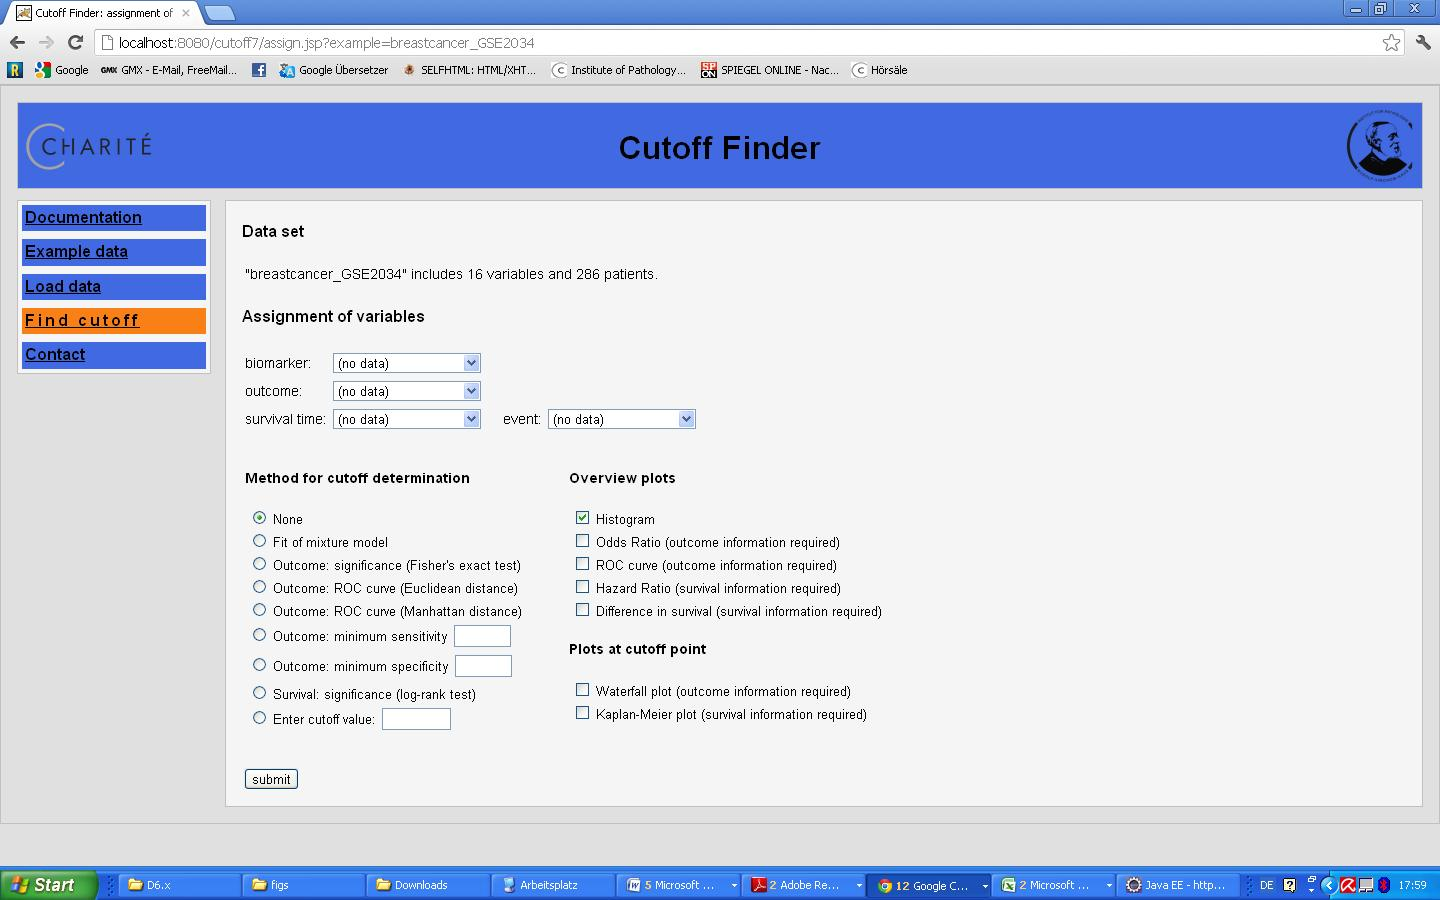
\includegraphics[width=0.9\textwidth]{fig1_screenshot_new}
\caption{\textbf{Screenshot of the Find cutoff webpage.} At the top of the webpage, the data set and the number of patients and variables in the data set is shown. At the middle the user can select the variables for analysis. At the bottom the user can choose the method for cutoff optimization and the set of plots to be generated.}
\label{fig:screenshot}
\end{figure}

\section{System architecture}
The webpages were implemented as Java Server Pages (JSPs).
All statistical analysis and visualization is executed using the statistical language R, a statistical and graphical environment suitable and common for the analysis of molecular data \cite{R}.
The JSPs connect to R using the package Rserve \cite{Rserve}.

\section{Data preparation and upload}
A data table can be uploaded for analysis
Molecule measurements, outcome and survival data should be stored in the columns, while each patient should belong to a row of the table.
Each column must have a header describing its content.
The maximum number of patients is 5000; the maximum number of variables is 50.
All table entries should be numeric.
Empty or string entries are treated as missing values.
The biomarker data can be on a metric or a ordinal level.
The table needs to be tab-separated, for example generated by saving a MS Excel document as .txt file.
After data upload, the user is automatically directed to the \emph{Find cutoff} webpage.

\section{Example data}
Alternatively to upload of own data, one of three example data sets can be imported into Cutoff Finder.
This can be done by a single mouse click on the \emph{Example data} webpage.
The example data include in the expression of three key genes in breast cancer tissues together with immunohistologically determined estrogen receptor status (ER\_IHC) and distance metastasis free survival (dmfs).
These data are part of larger microarray data sets that are publicly available from the Gene Expression Omnibus (GEO) repository.
Example analyses can be done by using one of the gene expression measurements as biomarker, ER\_IHC as outcome variable and dmfs\_time and dmfs\_event as survival time and survival event variables.
After data import, the user is automatically directed to the \emph{Find cutoff} webpage.

\section{Assignment of variables}
Selection of the variables for analysis can be done at the top of the \emph{Find cutoff} webpage.
Using dropdown menus, the columns of the data table can be assigned to biomarker, outcome
and survival variables.
A biomarker variable has to be selected, while selection of outcome and survival variables is optional.
All subsequent analyses are done using the selected variables.

\section{Methods for cutoff optimization}

The method for cutoff determination can be selected at the bottom of the \emph{Find Cutoff} webpage.
The optimal cutoff point as arithmetic mean of two succeeding values of the biomarker.
The first method optimizes the cutoff by fitting a mixture model to the distribution of the biomarker.
This method does not depend on outcome or survival information.
Further, there are five different methods that optimize the cutoff using the binary outcome variable.
Finally, a method is available for cutoff optimization using the survival variables.
Additional, it is possible to abstain from cutoff optimization or to use a manually defined cutoff.

\subsection{No cutoff point}
No cutoff optimization is done.
This method can be used to produce overview plots without marking of a cutoff point.

\subsection{Fit of mixture model}
A mixture model of two Gaussian distributions is fit to the histogram of the biomarker.
This procedure is implemented using the function \emph{flexmix} from the R package flexmix \cite{Leisch2004}.
The optimal cutoff is determined as the value where the probability density functions of the mixing distribution coincide.
When \emph{Histogram} is chosen as output plot, the fitted probability density functions and a vertical line indicating the cutoff point are added to the diagram (Figure~\ref{fig:histogram}).

\subsection{Outcome: significance}
This method correlates the dichotomized biomarker with a binary outcome variable using logistic regression.
Logistic regression is executed using the function \emph{glm} from R package stats \cite{R}.
The optimal cutoff is defined as the point with the most significant (Fisher's exact test) split.
Odds ratios (ORs) as well as sensitivity and specificity including 95\% confidence intervals are calculated.
Confidence intervals for proportions are estimated using Wilson's method as it is implemented in the R package binom \cite{binom}.

\subsection{Outcome: ROC curve}
Two methods determine the cutoff point by minimizing the distance on the ROC curve to the left top edge of the diagram.
The first method minimizes the Euclidean distance between these points.
In other words, the term $\sqrt{\mathrm{sensitivity}^2 + \mathrm{specificity}^2}$ is maximized.
The second method minimizes the Manhattan distance between the points.
Here, the sum of sensitivity and specificity is maximized, equivalent to maximization of Youden's $J$ statistics $J = \mathrm{sensitivity} + \mathrm{specificity} - 1$.

\subsection{Outcome: minimum sensitivity or specificity}
For each or these two methods, the user enters a percentage value.
The cutoff point is chosen as the first threshold for the biomarker where the sensitivity (or specificity) exceeds this predefined value.

\subsection{Survival: significance}
This method fits Cox proportional hazard models to the dichotomized variable and the survival variable.
Survival analysis is executed using the functions \emph{coxph} and \emph{survfit} from the R package survival \cite{survival}.
The optimal cutoff is defined as the point with the most significant (log-rank test) split.
Hazard ratios (HRs) including 95\% confidence intervals are calculated.

\subsection{Manual cutoff point}
The user manually chooses a cutoff point that is visualized in the overview plots.
Waterfall and/or Kaplan-Meier plots can be produced based on that cutoff.

\section{Plots}
Two different kinds of plots can be generated: overview plots and plots at the cutoff point.
Overview plots give a summary of all possible cutoff points with the optimal cutoff (determined by one of the methods described in the last section) marked by a vertical line.
The second kinds of plots are Waterfall and Kaplan-Meier plots that are build for a fixed cutoff point.
The set of plot to be generated can be chosen at the bottom of the \emph{Find cutoff} webpage.

In the following sections we present the zoo of plots that can be generated by Cutoff Finder.
Example plots are generated by importing the breast cancer data set GSE2034 and analyzing the
biomarker PGR 208205\_at with the outcome variable ER\_IHC and the survival variables
dmfs\_time and dmfs\_event.

\newpage

\begin{figure}[t]
\centering
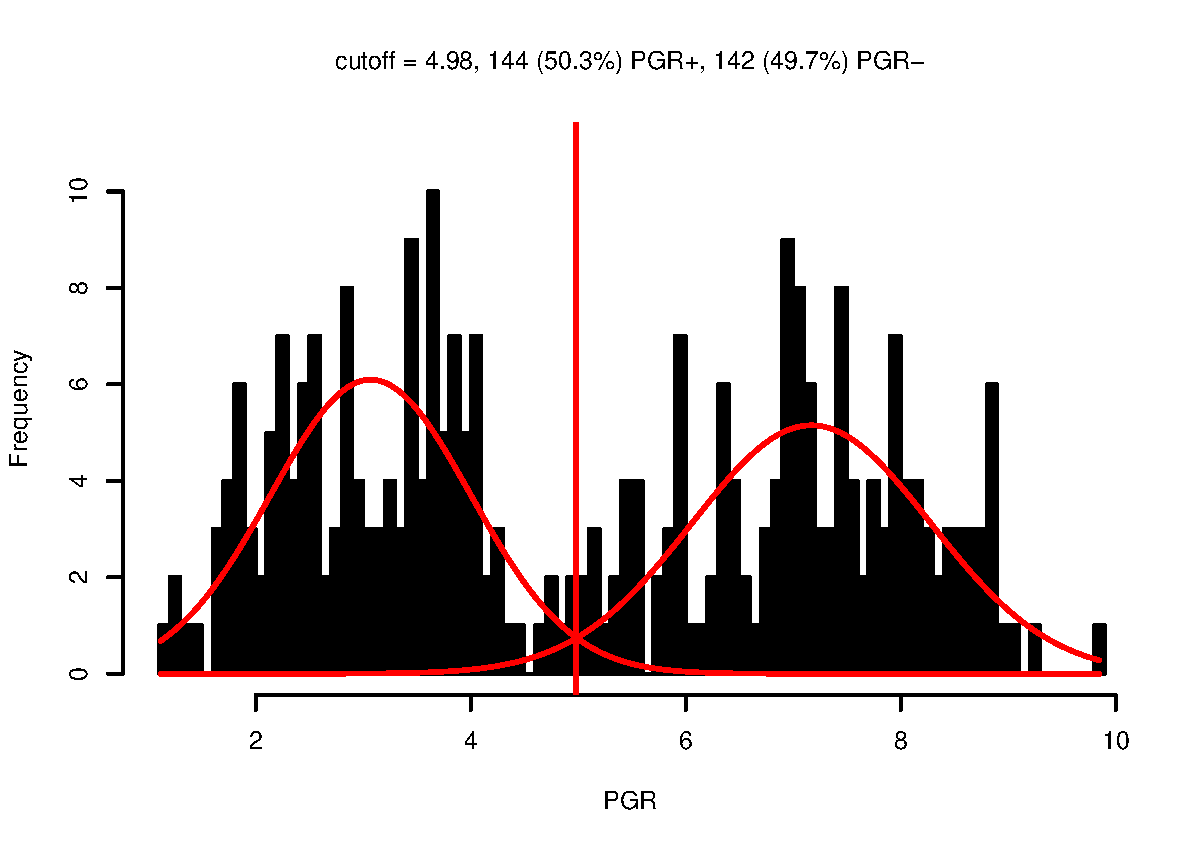
\includegraphics{Cutoff_Finder_manual-002}
\caption{\textbf{Histogram with fitted mixure model.}
Optimal cutoff point and the probability densities of the mixing distributions are shown as curves.}
\label{fig:histogram}
\end{figure}

\subsection{Histogram}
Figure~\ref{fig:histogram} shows a histogram of the biomarker with the optimal cutoff marked by a vertical line. The optimal cutoff depends on the method that was chosen for cutoff optimization.
Here, it was determined by fitting a mixture model to the distribution of the biomarker.
Additionally, the probability densities of the mixing distributions are shown as curves.

\newpage

\begin{figure}[t]
\centering
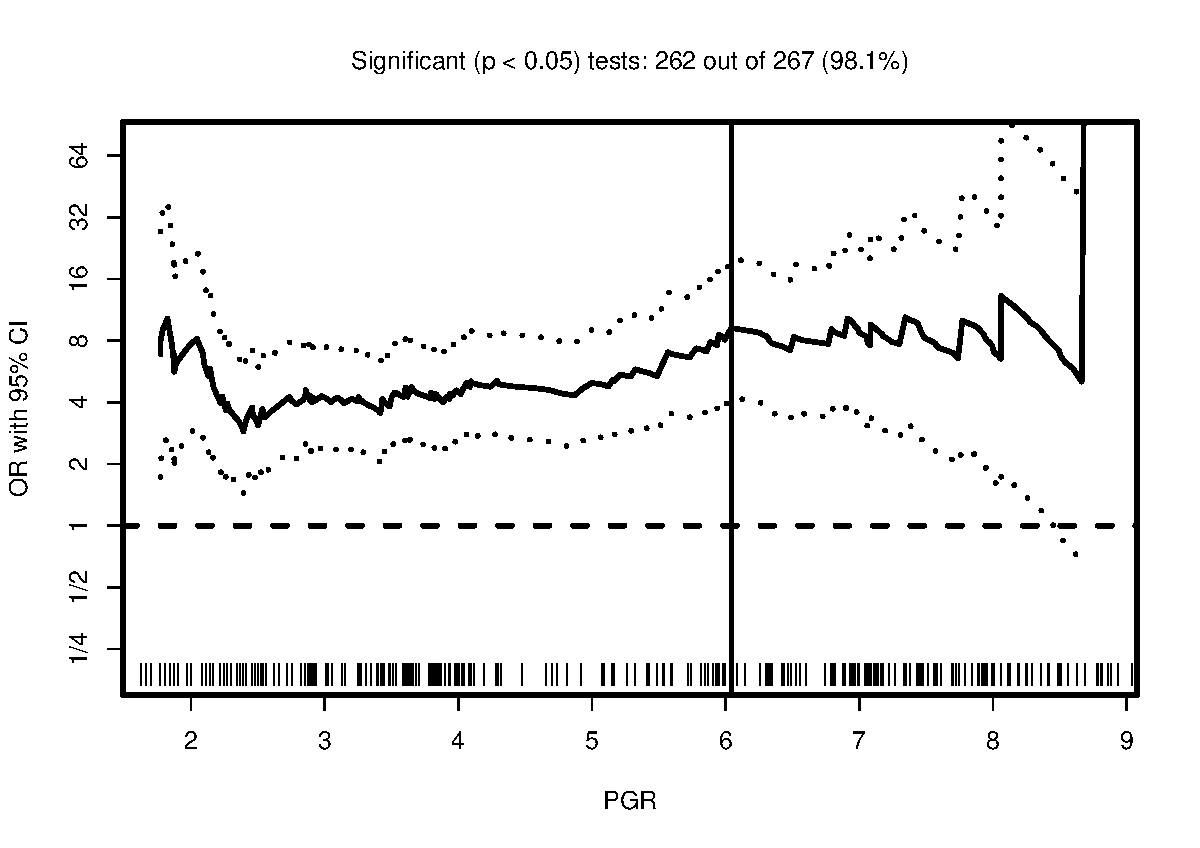
\includegraphics{Cutoff_Finder_manual-003}
\caption{\textbf{Odds ratio plot.}
The odds ratio (OR) including 95\% CI is shown in dependence of possible cutoff points.
The distribution of the biomarker is shown as rug plot at the bottom of the figure.}
\label{fig:or}
\end{figure}

\subsection{Odds ratio plot}
For each cutoff point, logistic regression of biomarker with respect to the outcome variable is executed.
The fits are done using the function \emph{glm} from the R package stat \cite{R}.
The resulting curve of odds ratios (ORs) is shown in Figure~\ref{fig:or}.
The percentage significant cutoffs out of all investigated cutoffs is displayed at the top of the figure.

The optimal cutoff is marked by a vertical line.
The optimal cutoff depends on the method that was chosen for cutoff optimization.
Here, we optimized the cutoff by maximizing the significance assessed by Fisher's exact test.

\newpage

\begin{figure}[t]
\centering
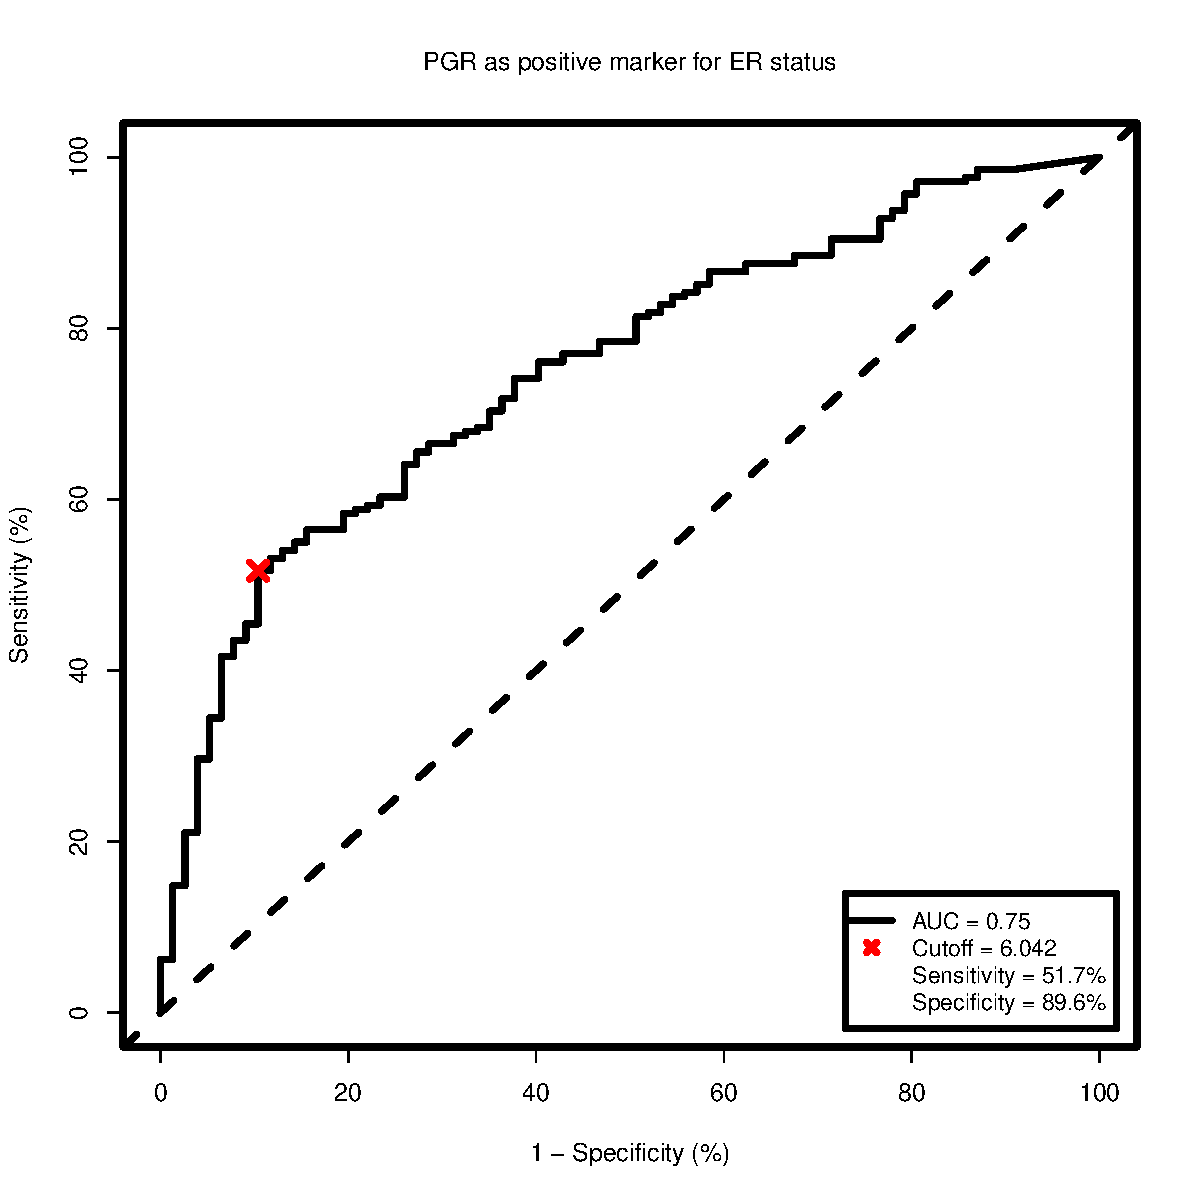
\includegraphics{Cutoff_Finder_manual-004}
\caption{\textbf{ROC curve with optimal cutoff point.}
The quality of the prediction can be assessed by the area under the curve (AUC) and sensitivity and specificity at the cutoff point.}
\label{fig:roc}
\end{figure}

\subsection{ROC curve}

ROC curves are the standard method to balance between sensitivity and specificity of a molecular test.
Figure~\ref{fig:roc} shows the ROC curve for the prediction of immunohistological estrogene receptor status by progesterone receptor expression.
The quality of the prediction can be assessed by the area unnder the curve (AUC) and the values for sensitivity and specificity at the cutoff point.

The optimal cutoff is marked by a red cross.
The optimal cutoff depends on the method that was chosen for cutoff optimization.
Here, we optimized the cutoff by maximizing the significance assessed by Fisher's exact test.

\newpage

\begin{figure}[t]
\centering
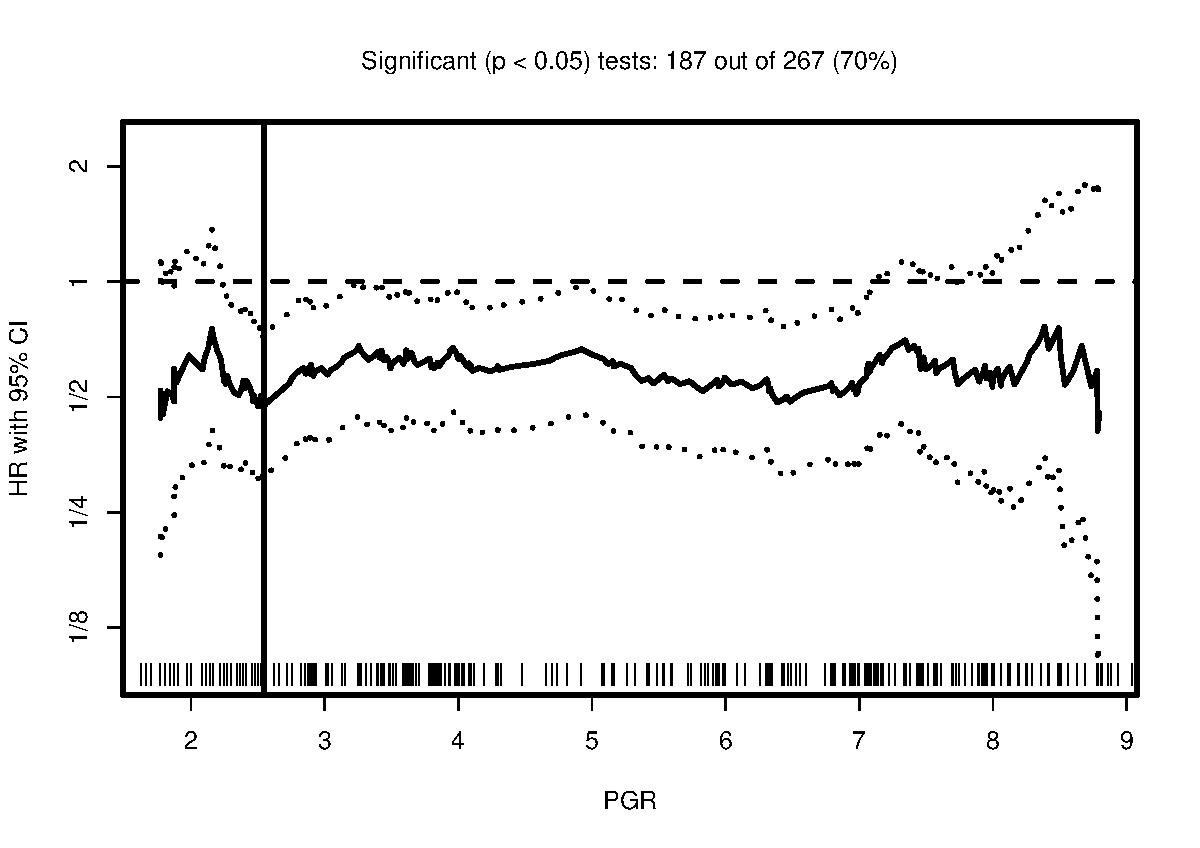
\includegraphics{Cutoff_Finder_manual-005}
\caption{\textbf{Hazard ratio plot.}
The hazard ratio (HR) with 95\% CI is shown in dependence of possible cutoff points.
The distribution of the biomarker is shown as rug plot at the bottom of the figure.}
\label{fig:hr}
\end{figure}

\subsection{Hazard ratio plot}
For each cutoff point, a Cox analyis of biomarker and the survival variable is executed.
The fits are done using the functions \emph{coxph} and \emph{survfit} from the R package survival \cite{survival}.
The resulting curve of hazard ratios (HRs) is shown in Figure~\ref{fig:hr}.
The percentage significant cutoffs out of all investigated cutoffs is displayed at the top of the figure.

The optimal cutoff is marked by a vertical line.
The optimal cutoff depends on the method that was chosen for cutoff optimization.
Here, we optimized the cutoff by maximizing the significance assessed by the log-rank test.

\newpage

\begin{figure}[t]
\centering
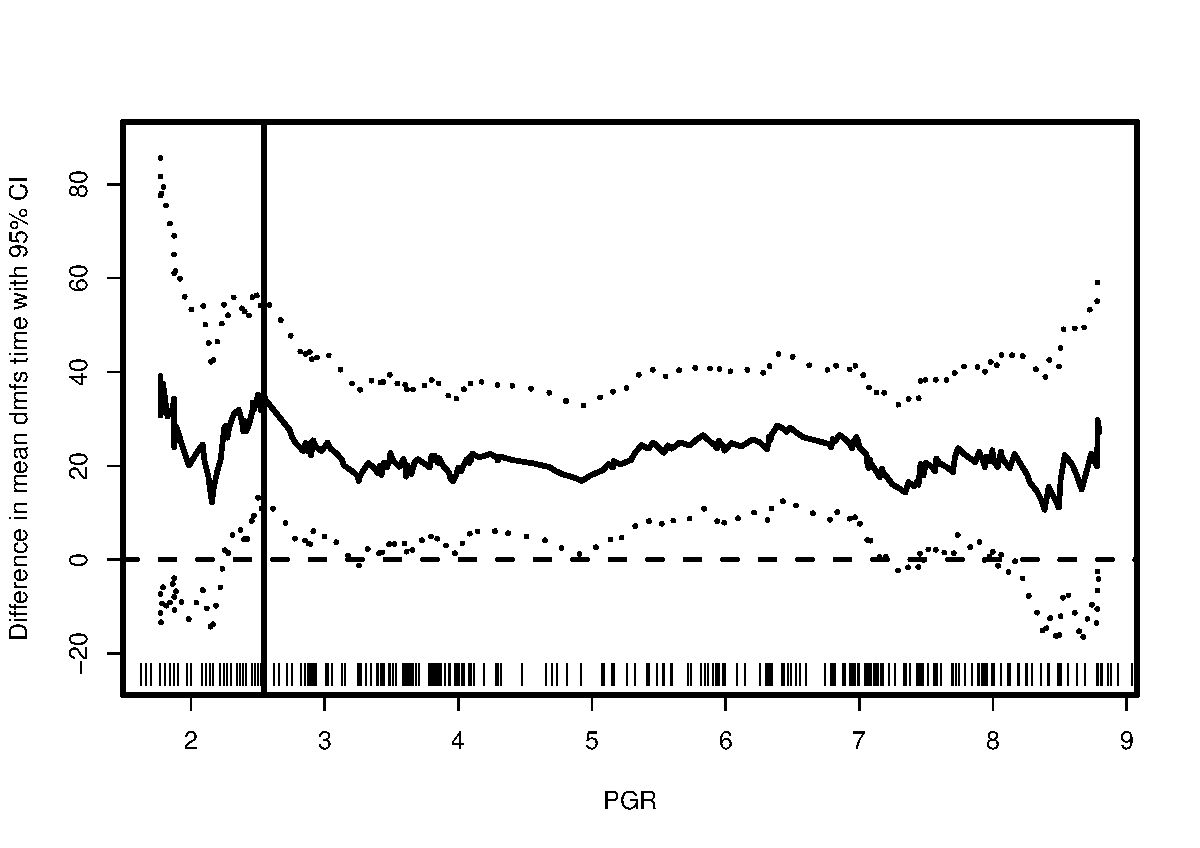
\includegraphics{Cutoff_Finder_manual-006}
\caption{\textbf{Plot of the differences in survival time.}
The mean survival time is estimated in the samples where the biomarker is highly expressed
and in the samples where the biomarker is lowly expressed.
The difference of the mean survival times including is plotted.
The distribution of the biomarker is shown as rug plot at the bottom of the figure.}
\label{fig:diff}
\end{figure}

\subsection{Differences in survival time}
For each cutoff point, the mean survival time for both subcohorts is estimated using the function \emph{survfit} from the R package survival \cite{survival}.
The estimate for the mean survival time is the area under the Kaplan-Meier curve.
To avoid divergent integrals, a time endpoint has to be chosen for calculation of the area.
Here, all mean survival times are estimated using the maximum time occuring in the data.
Then, the difference of the mean survival times of the two subcohorts is calculated.
The resulting survival time curve is shown in Figure~\ref{fig:diff}.

The optimal cutoff is marked by a vertical line.
The optimal cutoff depends on the method that was chosen for cutoff optimization.
Here, we optimized the cutoff by maximizing the significance assessed by the log-rank test.

\newpage

\begin{figure}[t]
\centering
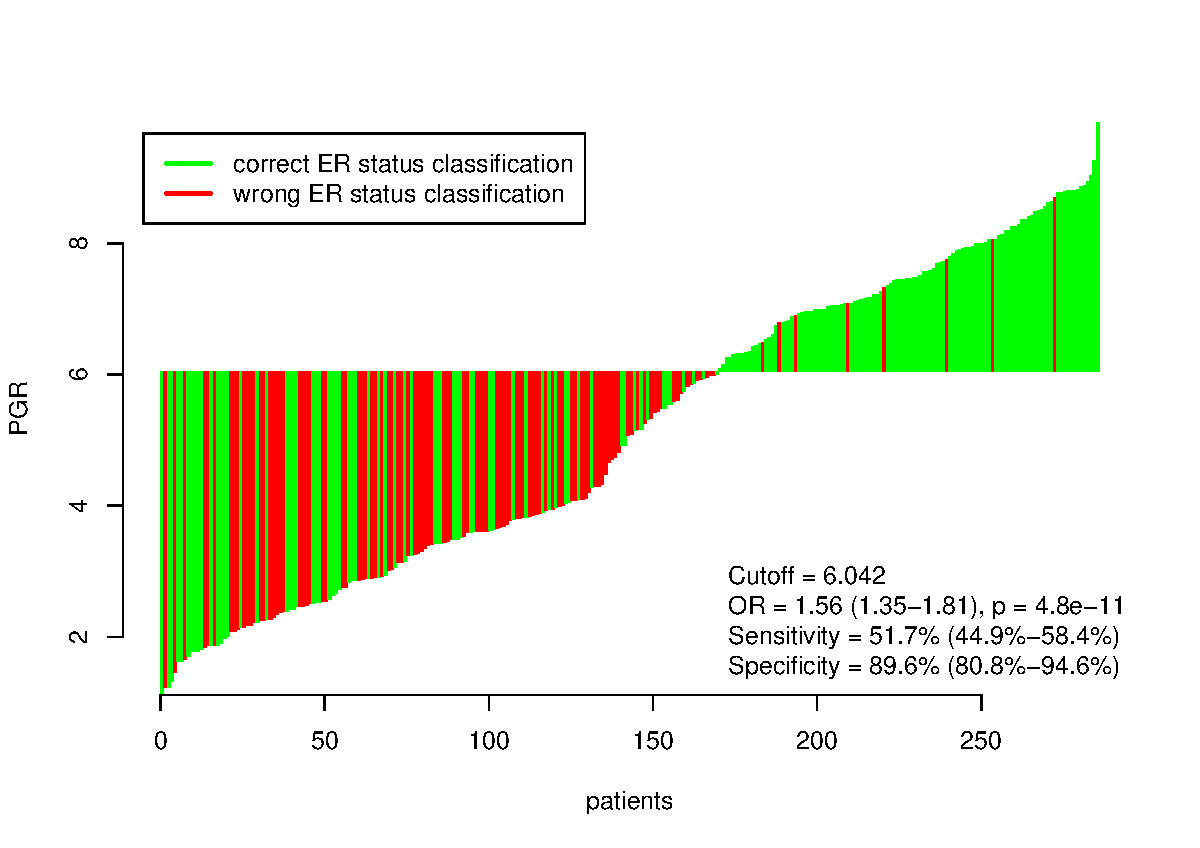
\includegraphics{Cutoff_Finder_manual-007}
\caption{\textbf{Waterfall plot.}
The plot shows all the samples ordered by the value of the biomarker.
The color encodes agreement of the biomarker and the reference classification (green bars)
or disagreement of the biomarker and the reference classification (red bars).}
\label{fig:waterfall}
\end{figure}

\subsection{Waterfall plot}
Figure~\ref{fig:waterfall} shows a waterfall plot a the optimal cutoff point.
The optimal cutoff depends on the method that was chosen for cutoff optimization.
Here, we optimized the cutoff by maximizing the significance assessed by Fisher's exact test.

A couple of quantities associated with the split induced by the cutoff point are printed at the bottom of the figure:
The odds ratio (OR) is estimated by logistic regression using the function \emph{glm} from the R package stats \cite{R}.
A $p$-value is calculated using Fisher's exact test.
95\% confidence intervals of sensitivity and specificity are estimated using Wilson's methods as it is implemented in the function \emph{binom.conf} from the R package binom \cite{binom}.

\newpage

\begin{figure}[t]
\centering
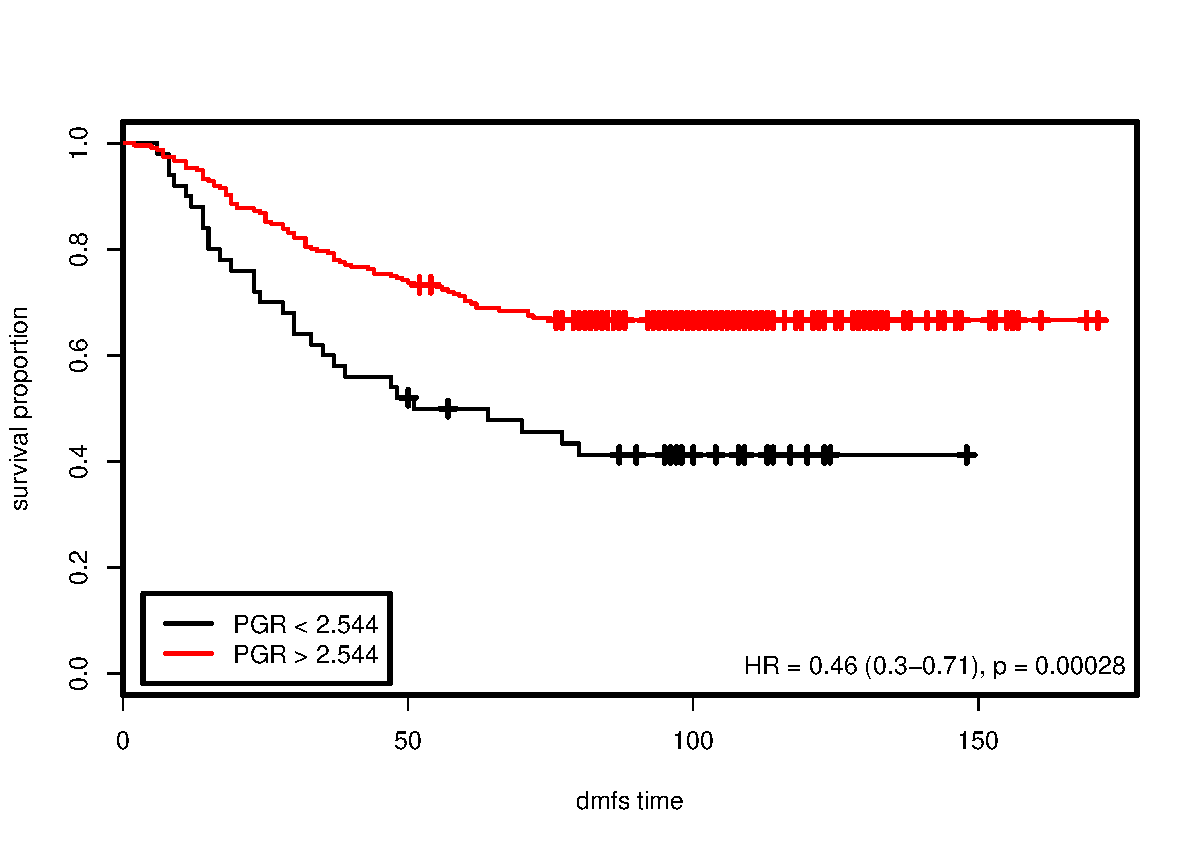
\includegraphics{Cutoff_Finder_manual-008}
\caption{\textbf{Kaplan-Meier plot.}
Survival analysis was executed at the optimal cutoff.
The hazard ratio (HR) includung 95\% CI is estimated using Cox proportional hazard modeling. The $p$-value is calculated using the log-rank test.}
\label{fig:km}
\end{figure}

\subsection{Kaplan-Meier plot}
A Kaplan-Meier plot at the optimal cutoff point is shown in Figure~\ref{fig:km}.
The optimal cutoff depends on the method that was chosen for cutoff optimization.
Here, we optimized the cutoff by maximizing the significance assessed by the log-rank test.
Kaplan-Meier analysis is executed using the function \emph{survfit} from the R package survival \cite{survival}.

\section{Shiny app}
The shiny app can be used as in the following example:

\begin{lstlisting}[language=R]
# To load the library
library(CutoffFinder)

# using default port
runCutoffFinder()
\end{lstlisting}

\newpage

\bibliographystyle{unsrt}
\bibliography{Cutoff_Finder_manual}

\end{document}
